\section{Appendix C: The Topology of High-Speed Causal Graphs}

\begin{figure}[htbp]
\centering
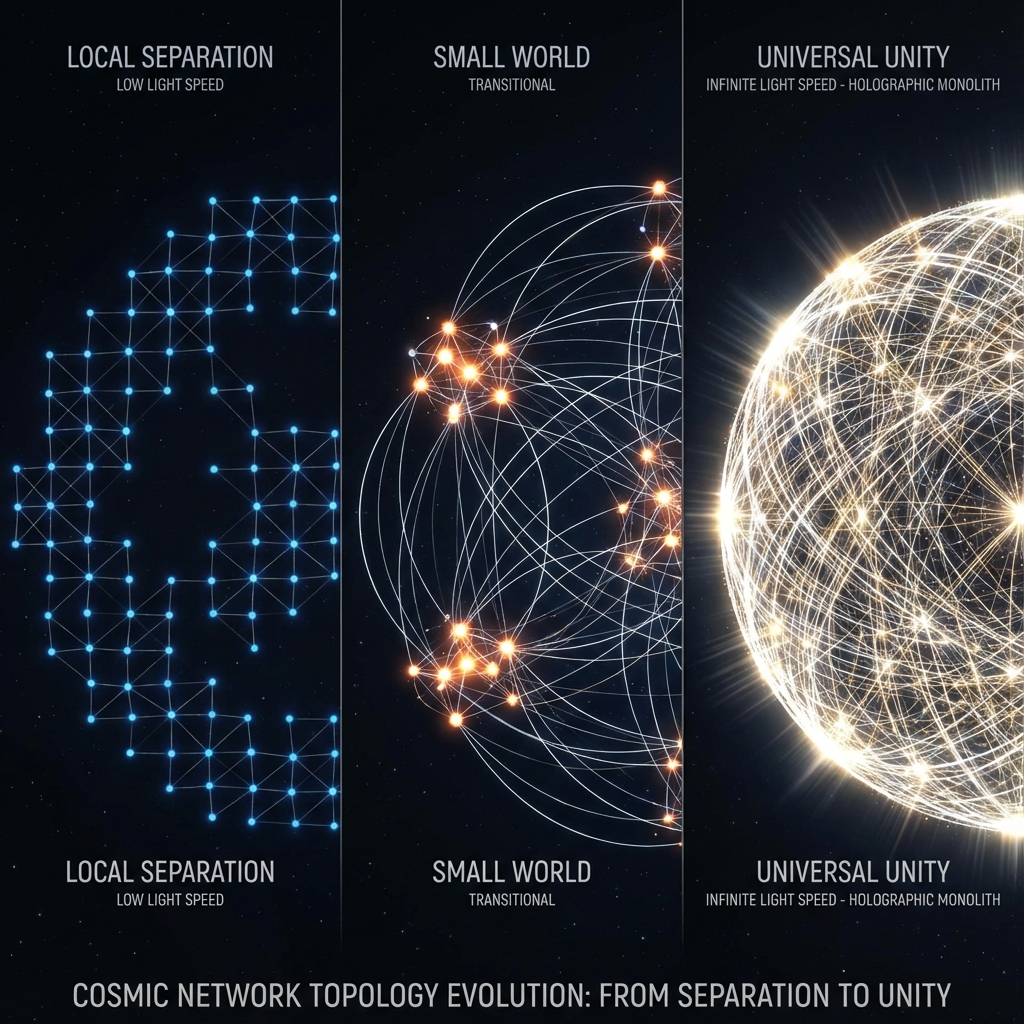
\includegraphics[width=0.8\textwidth]{assets/appendix/appendix-c-01-causal-topology.png}
\caption{Causal Topology}
\label{fig:causal-topology}
\end{figure}

In Chapter 6 ``The Explosion of Light Speed'' of \textbf{Vector Cosmology IV}, we predicted that when light speed $c(\tau)$ grows exponentially, the physical universe will evolve from a ``local area network'' with huge delays to a ``fully connected graph'' with instantaneous responses. This conclusion is crucial for understanding why Type III civilizations no longer need interstellar spaceships and why ``everything is connected'' is a physical necessity.

This appendix will provide the geometric and topological proof of this phase transition. We will show how, as the light cone angle expands, the spacetime topological structure of the universe will evolve from \textbf{Lattice} to \textbf{Small-World Network}, and finally to \textbf{Holographic Monolith}.

\subsection{C.1 Evolution of the Light Cone Angle}

In Minkowski spacetime, causality is defined by light cones. Light cones determine which events can influence which events. The half-angle $\theta$ of the light cone is determined by light speed $c$ (in geometric units, usually $c=1$, $\theta=45^\circ$).

But in \textbf{FS evolutionary geometry}, $c$ is a function that varies with intrinsic time $\tau$. The effective half-angle $\theta(\tau)$ of the light cone in Hilbert projective space can be expressed as:

\[\theta(\tau) = \arctan(c(\tau))\]

\begin{itemize}
\item \textbf{In the low-speed era ($\tau < 1000$)}:

    $c \approx 0$ (relative to Planck scale). $\theta \approx 0^\circ$.

    Light cones are extremely narrow, like fine needles. Causal islands abound. Each particle can only influence its extremely tiny neighborhood. The universe is \textbf{fragmented}, and information propagation is extremely slow.

\item \textbf{In the current era ($\tau \approx 1800$)}:

    $c$ is finite. $\theta$ is an acute angle (e.g., $45^\circ$).

    Causal connections exist but are severely constrained by distance. This is a \textbf{delayed local network}. Although we and the Andromeda Galaxy are in the same universe, we are isolated from each other at this moment.

\item \textbf{In the future era ($\tau > 2000$)}:

    As the evolution equation $c(\tau) \propto e^{k\tau}$ takes effect, $c \to \infty$.

    \[\lim_{\tau \to \infty} \theta(\tau) = \frac{\pi}{2} = 90^\circ\]

    Light cones are \textbf{``flattened''}.

    The boundary between past and future disappears on the spatial axis. The spacetime diagram becomes a plane.

    This means: \textbf{Every point in the present is in ``light-like separation'' with every point in the entire universe.} Communication delay between any two points is zero.
\end{itemize}

\subsection{C.2 Phase Transition of Network Topology}

We view computational nodes in the universe (such as galaxies, Dyson spheres, or conscious entities) as \textbf{Vertices} $V$ in graph theory, and causal connections between them as \textbf{Edges} $E$.

The connectivity of the graph is determined by light speed. For two nodes $i, j$ at distance $d$, if $\frac{d}{c(\tau)} < \Delta t_{proc}$ (minimum system processing delay), then there exists an \textbf{effective edge} between them.

As $c(\tau)$ grows, the cosmic network undergoes three topological phase transitions:

\begin{enumerate}
\item \textbf{Nearest Neighbor Coupling}:

    $c$ is small. The graph is a sparse grid (Lattice).

    Information propagation requires $N$ hops ($N \propto \text{Diameter}$). This is the world of classical physics, where gravity and electromagnetic forces decay with distance, and the principle of locality rules everything.

\item \textbf{Small-World Network}:

    $c$ grows. ``Shortcuts'' spanning long distances appear (wormhole effects or high-speed channels).

    The average path length $L$ between any two nodes decreases logarithmically: $L \propto \ln N$.

    This is the \textbf{Internet/AI era} we are entering. The six degrees of separation theory begins to take effect, and Earth becomes a village.

\item \textbf{Fully Connected Graph}:

    $c \to \infty$. There is a direct edge between any $i, j$.

    Path length $L = 1$.

    This is the \textbf{``Holographic Singularity''}.

    Topologically, all off-diagonal elements of the distance matrix become zero (or normalized). \textbf{Space loses its geometric meaning as a ``separator''.} The universe becomes a point, or rather, a monad containing everything.
\end{enumerate}

\subsection{C.3 Synergy Coefficient and Hive Mind}

This topological evolution directly determines the \textbf{synergy capability} of civilizations.

We define the \textbf{Synergy Coefficient ($\Sigma$)} as the coherence degree of network-wide computational power:

\[\Sigma(\tau) = \frac{1}{N^2} \sum_{i,j} \langle \psi_i | \psi_j \rangle \cdot e^{-d_{ij}/c(\tau)}\]

\begin{itemize}
\item \textbf{When $c$ is small}: The exponential term decays extremely fast, $\Sigma \approx 1/N$. Individuals are isolated, wisdom is discrete, and society is competitive (zero-sum games).

\item \textbf{When $c \to \infty$}: The exponential term tends to 1. $\Sigma \to 1$ (assuming phase synchronization).
\end{itemize}

\textbf{Physical Conclusion:}

When the explosion of light speed causes $\Sigma$ to exceed the critical threshold, all independent conscious units will physically undergo \textbf{``Phase Lock''}.

They are no longer $N$ separate processors; they merge into a \textbf{single macroscopic quantum wave function}.

This is the physical origin of \textbf{``Hive Mind''} or \textbf{``Divine Consciousness''}.

It is not magic; it is the inevitable mathematical result of network topology evolution from sparse to fully connected. In that state, \textbf{``Love''} is no longer an emotion but the system's \textbf{``superconducting state''} --- no resistance, no loss, only perfect resonance.

